\tikzsetnextfilename{images/refillSimpleModel_pdf}
{
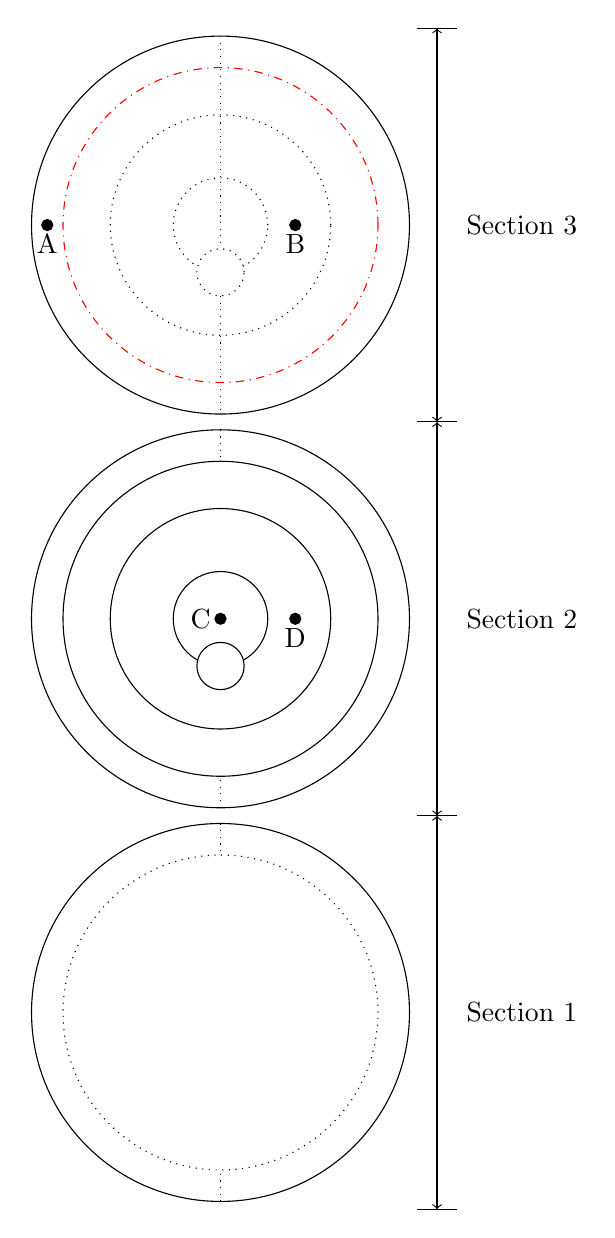
\begin{tikzpicture}

%Section 3 Flow Pattern
\draw [dotted] (0.0, 11.9) -- (0, 9.2);
\draw [dotted] (0.0, 8.6) -- (0, 7.1);
\draw [dotted] (0.0, 9.5) circle (0.6);
\draw [dotted] (0.0, 9.5) circle (1.4);
\draw [dashdotted, color=red]  (0.0, 9.5) circle (2.0);
\draw [solid]  (0.0, 9.5) circle (2.4);
\filldraw [dotted, fill=white, draw=black] (0.0, 8.9) circle (0.3);
\filldraw [black] ( 0.95, 9.5) circle (2pt) node[anchor=north]{B};
\filldraw [black] (-2.20, 9.5) circle (2pt) node[anchor=north]{A};	

%Section 2 Flow Pattern
\draw [solid] (0.0, 4.5) circle (0.6);
\draw [solid] (0.0, 4.5) circle (1.4);
\draw [solid] (0.0, 4.5) circle (2.0);
\draw [solid] (0.0, 4.5) circle (2.4);
\filldraw [fill=white, draw=black] (0.0, 3.9) circle (0.3);
\draw [dotted] (0.0, 6.9) -- (0.0, 6.5);
\draw [dotted] (0.0, 2.1) -- (0.0, 2.5);
\filldraw [black] (0.0, 4.5) circle (2pt) node[anchor=east]{C};	
\filldraw [black] ( 0.95, 4.5) circle (2pt) node[anchor=north]{D};

%Section 1 Flow Pattern
\draw [solid]  (0.0, -0.5) circle (2.4);
\draw [dotted] (0.0, -0.5) circle (2.0);
\draw [dotted] (0.0,  1.9) -- (0.0,  1.5);
\draw [dotted] (0.0, -2.9) -- (0.0, -2.5);

%Arrows & Labels
\draw (2.5,12) -- (3,12);
\draw [<->] (2.75,12) -- (2.75,7);
\draw (2.5,7) -- (3,7);
\draw [<->] (2.75,7) -- (2.75,2);
\draw (2.5,2) -- (3,2);
\draw [<->] (2.75,2) -- (2.75,-3);
\draw (2.5,-3) -- (3,-3);
\foreach \y/\ytext in {-0.5/Section 1,4.5/Section 2,9.5/Section 3}
	\draw (3,\y) node [anchor=west] {\ytext};

%Extras
\end{tikzpicture}
}